\subsection[\textless{}T\textgreater]{Templates}

\begin{frame}[fragile]
  \frametitlecpp[98]{Templates}
  \begin{block}{Concept}
    \begin{itemize}
    \item The \cpp way to write reusable code
      \begin{itemize}
        \item aka macros on steroids
      \end{itemize}
    \item Applicable to functions and objects
    \end{itemize}
  \end{block}
  \begin{cppcode}
    template<typename T>
    const T & max(const T &A, const T &B) {
      return A > B ? A : B;
    }

    template<typename T>
    struct Vector {
      int m_len;
      T* m_data;
    };
 \end{cppcode}
\end{frame}

\begin{frame}[fragile]
  \frametitlecpp[98]{Templates}
  \begin{alertblock}{Warning}
    These are really like macros
    \begin{itemize}
      \item they are compiled n times
      \item they need to be defined before used
      \begin{itemize}
        \item so all templated code has to be in headers
      \end{itemize}
      \item this may lead to longer compilation times and bigger libraries
    \end{itemize}
  \end{alertblock}
  \newsavebox{\codepiece}
  \begin{lrbox}{\codepiece}
    \begin{minipage}{.35\linewidth}
      \small
      \begin{cppcode*}{gobble=4}
        template<typename T>
        T func(T a) {
          return a;
        }
      \end{cppcode*}
    \end{minipage}
  \end{lrbox}
  \newsavebox{\codepiecea}
  \begin{lrbox}{\codepiecea}
    \begin{minipage}{.4\linewidth}
      \small
      \begin{cppcode*}{gobble=4,linenos=false}
        int func(int a) {
          return a;
        }
      \end{cppcode*}
    \end{minipage}
  \end{lrbox}
  \newsavebox{\codepieceb}
  \begin{lrbox}{\codepieceb}
    \begin{minipage}{.4\linewidth}
      \small
      \begin{cppcode*}{gobble=4,linenos=false}
        double func(double a) {
          return a;
        }
      \end{cppcode*}
    \end{minipage}
  \end{lrbox}
  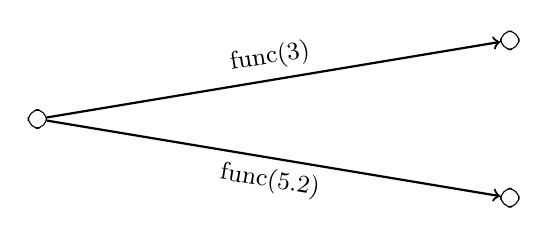
\begin{tikzpicture}[rectangle,rounded corners]
    \draw node (template) [draw] {\usebox{\codepiece}}
          node (templatea) [draw] at (6cm,+1cm) {\usebox{\codepiecea}}
          node (templateb) [draw] at (6cm,-1cm) {\usebox{\codepieceb}};
    \draw[->,thick] (template) -- (templatea) node [above,midway,sloped] {\small func(3)};
    \draw[->,thick] (template) -- (templateb) node [below,midway,sloped] {\small func(5.2)};
  \end{tikzpicture}
\end{frame}

\begin{frame}[fragile]
  \frametitlecpp[98]{Templates}
  \begin{block}{Arguments}
    \begin{itemize}
    \item can be a class,
    \item you can have several
    \item last ones can have a default value
    \end{itemize}
  \end{block}
  \begin{cppcode*}{}
    template<typename KeyType=int, typename ValueType=KeyType>
    struct Map {
      void set(const KeyType &key, ValueType value);
      ValueType get(const KeyType &key);
    }

    Map<std::string, int> m1;
    Map<float> m2;   // Map<float, float>
    Map<> m3;        // Map<int, int>
  \end{cppcode*}
\end{frame}

\begin{frame}[fragile]
  \frametitlecpp[98]{Templates implementation}
  \begin{cppcode*}{}
    template<typename KeyType=int, typename ValueType=KeyType>
    struct Map {
      void set(const KeyType &key, ValueType value);
      ValueType get(const KeyType &key);
    }

    template<typename KeyType, typename ValueType>
    void Map<KeyType, ValueType>::set
       (const KeyType &key, ValueType value) {
      ...
    }

    template<typename KeyType, typename ValueType>
    ValueType Map<KeyType, ValueType>::get
       (const KeyType &key) {
      ...
    }
  \end{cppcode*}
\end{frame}

\begin{frame}[fragile]
  \frametitle{Non-type template parameter \hfill \cpp98 / \cpp17 / \cpp20}
  \begin{block}{template parameters can also be a value}
    \begin{itemize}
    \item integral types, pointer, enums in \cpp98
    \item auto in \cpp17
    \item floats and literals in \cpp20
    \end{itemize}
  \end{block}
  \begin{cppcode*}{}
    template<unsigned int N> struct Polygon {
      Polygon(float radius);
      float perimeter() {return 2*N*sin(PI/N)*m_radius;}
      float m_radius;
    };
  \end{cppcode*}
\end{frame}

\begin{frame}[fragile]
  \frametitlecpp[98]{Templates}
  \begin{block}{Specialization}
    templates can be specialized for given values of their parameter
  \end{block}
  \begin{cppcode*}{}
    template<typename F, unsigned int N> struct Polygon {
      Polygon(F radius) : m_radius(radius) {}
      F perimeter() {return 2*N*sin(PI/N)*m_radius;}
      F m_radius;
    };

    template<typename F>
    struct Polygon<F, 6> {
      Polygon(F radius) : m_radius(radius) {}
      F perimeter() {return 6*m_radius;}
      F m_radius;
    };
  \end{cppcode*}
\end{frame}

\begin{frame}[fragile]
  \frametitlecpp[98]{The full power of templates}
  \begin{alertblock}{Exercise Time}
    \begin{itemize}
    \item go to code/templates
    \item look at the OrderedVector code
    \item compile and run playwithsort.cpp. See the ordering
    \item modify playwithsort.cpp and reuse OrderedVector with Complex
    \item improve OrderedVector to template the ordering
    \item test reverse ordering of strings (from the last letter)
    \item test order based on {\color{blue} \href{https://en.wikipedia.org/wiki/Taxicab_geometry}{Manhattan distance}} with complex type
    \item check the implementation of Complex
    \item try ordering complex of complex
    \end{itemize}
  \end{alertblock}
\end{frame}
